\section{Polar Coordinate System}

As an alternative to the Cartesian coordinate system there exists the polar coordinate system. A (two dimensional) polar coordinate is described by a rotation and a radius. Like the Cartesian coordinate system we need to define a base grid with an origin and orientation, see figure \ref{fig:polar-coordinate-system}.

\begin{figure}[H]
\centering
    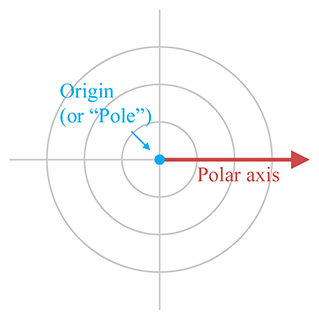
\includegraphics{07_polar_coordinate_system}
\caption{Polar coordinate system}
\label{fig:polar-coordinate-system}
\end{figure}

\subsection{Two dimensional polar coordinates}

The steps to take to find a polar coordinate $(r,\theta)$ are as follows: 

\begin{enumerate}
	\item Start at the origin facing the polar axis. Then rotate by the angle $\theta$, where a positive $\theta$ usually means counter clockwise rotation.
	\item Now move forward from the origin by a distance of $r$ units.
\end{enumerate}

\begin{figure}[H]
\centering
    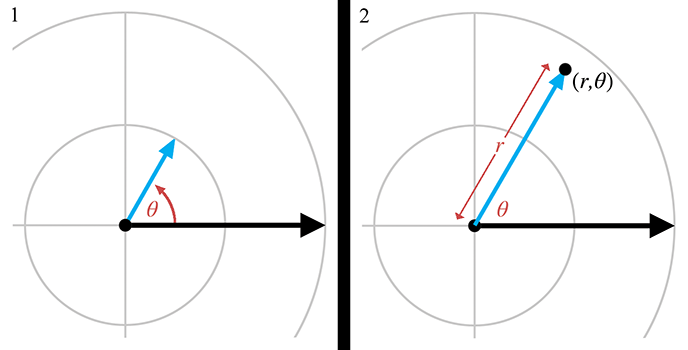
\includegraphics{07_2d_polar_coordinate}
\caption{Locating 2D polar coordinate}
\label{fig:locating-2d-polar-coordinate}
\end{figure}

\subsubsection{Canonical form}

As you might have noticed there exists aliasing of coordinates. For example, adding $2\pi$ to $\theta$ is aliases the original $\theta$. To avoid aliasing issues polar coordinates can be turned into canonical form:

\begin{itemize}
	\item $r \geq 0$, we don't measure distances "backwards".
	\item $-180^\circ < \theta \leq 180^\circ$, the angle is limited to half a revolution.
	\item $r=0 \implies \theta=0$, at the origin, set the angle to $0$.
\end{itemize}

An example C implementation can be found in the \path{code/} subdirectory with filename \path{07_canonical_2d_polar_coordinates.c}.

\subsubsection{Polar coordinate to Cartesian coordinate}

$$
\begin{array}{lr}
x=r\cos\theta; & y=r\sin\theta.
\end{array}
$$

\subsubsection{Cartesian coordinate to Polar coordinate}

$$
\begin{array}{lr}
r=\sqrt{x^2+y^2}; & \theta=\text{atan2}(y,x).
\end{array}
$$

Refer the book for a more depth explanation why we use $\text{atan2}$ rather than $\arctan$. An example C implementation can be found in the \path{code/} subdirectory with filename \path{07_2d_cartesian_to_polar.c}.

\subsubsection{atan2}

$\text{atan2}$ is a useful function to handle edge cases of $\arctan$. The following definition is roughly how it works in most computer languages. The exception being that $\text{atan2}$ is usually not defined for $(0,0)$, but for ease of use we do make this assumption. Furthermore, remember that the argument order is $y$ followed by $x$. Speaking from experience this is an easy mistake to make.

\begin{equation*}
	\text{atan2}(y,x) =
	\begin{cases}
		0, & x=0,y=0, \\
		+90^\circ, & x=0,y>0, \\
		-90^\circ, & x=0,y<0, \\
		\arctan(y/x), & x>0, \\
		\arctan(y/x)+180^\circ, & x<0,y\geq 0 \\
		\arctan(y/x)-180^\circ, & x<0,y<0
	\end{cases}
\end{equation*}

\subsection{Three dimensional polar coordinates}

The concept of polar coordinates can be extended to three dimensions in two distinct ways: cylindrical and spherical coordinates.

\subsection{Cylindrical coordinates}

The first type of the three dimensional polar coordinate is the cylindrical coordinate. The base of the cylinder is defined by a two dimensional polar coordinate, while the third coordinate is an axis like in Cartesian systems.

\begin{figure}[H]
\centering
    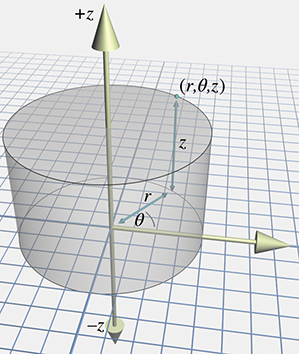
\includegraphics{07_cylindrical_coordinates}
\caption{Cylindrical coordinates}
\label{fig:cylindrical-coordinates}
\end{figure}

\subsubsection{Cylindrical coordinate to Cartesian coordinate}

$$
\begin{array}{lcr}
x=r\cos\theta; & y=r\sin\theta; & z=z.
\end{array}
$$

\subsubsection{Cartesian coordinate to Cylindrical coordinate}

$$
\begin{array}{lcr}
r=\sqrt{x^2+y^2}; & \theta=\text{atan2}(y,x); & z=z.
\end{array}
$$

\subsection{Spherical coordinates}

Unlike cylindrical coordinates, spherical coordinates are a bit more complex and require a bit more computation. A spherical coordinate is defined by two angles and a radius.

\begin{figure}[H]
\centering
    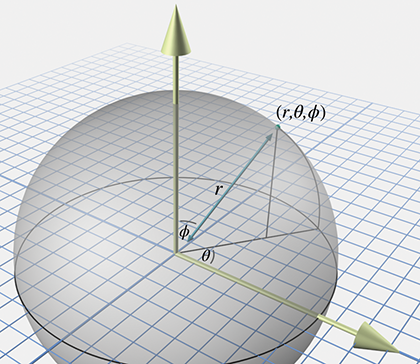
\includegraphics{07_spherical_coordinates}
\caption{Spherical coordinates}
\label{fig:spherical-coordinates}
\end{figure}

\subsubsection{Canonical Spherical coordinates}

Spherical coordinates has even more issues with regards to aliasing. So once again we define some common rules to avoid this. Where $\theta$ is replaced with the letter $h$ for heading, and $\phi$ replaced with the letter $p$ for pitch:

\begin{itemize}
	\item $r \geq 0$, we don't measure distances "backwards".
	\item $-180^\circ < h \leq 180^\circ$, the heading is limited to half a revolution.
	\item  $-90^\circ \leq p \leq 90^\circ$, pitch limits are straight up and down.
	\item $r=0 \implies h=p=0$, at the origin set the angles to $0$.
	\item $|p|=90^\circ \implies h=0$, when looking up or down set heading to $0$.
\end{itemize}

An example C implementation can be found in the \path{code/} subdirectory with filename \path{07_canonical_spherical_coordinates.c}.

\subsubsection{Canonical Spherical coordinate to Cartesian coordinate}

$$
\begin{array}{lcr}
x=r\cos p \sin h; & y=-r\sin p; & z=\cos p \cos h.
\end{array}
$$

\subsubsection{Cartesian coordinate to Canonical Spherical coordinate}

$$
\begin{array}{lcr}
r=\sqrt{x^2+y^2+z^2}; & h=\text{atan2}(x,z); & p=\arcsin(-y/r).
\end{array}
$$

An example C implementation can be found in the \path{code/} subdirectory with filename \path{07_3d_cartesian_to_spherical.c}.
